\documentclass[twocolumn, amsmath, amsfonts, amssymb]{aastex62}
\usepackage{mathtools}
\usepackage{bm}
\newcommand{\vdag}{(v)^\dagger}
\newcommand\aastex{AAS\TeX}
\newcommand\latex{La\TeX}

\newcommand{\Div}[1]{\ensuremath{\nabla\cdot\left( #1\right)}}
\newcommand{\DivU}{\ensuremath{\nabla\cdot\bm{u}}}
\newcommand{\angles}[1]{\ensuremath{\left\langle #1 \right\rangle}}
\newcommand{\KS}[1]{\ensuremath{\text{KS}(#1)}}
\newcommand{\KSstat}[1]{\ensuremath{\overline{\text{KS}(#1)}}}
\newcommand{\grad}{\ensuremath{\nabla}}
\newcommand{\RB}{Rayleigh-B\'{e}nard }
\newcommand{\stressT}{\ensuremath{\bm{\bar{\bar{\Pi}}}}}
\newcommand{\lilstressT}{\ensuremath{\bm{\bar{\bar{\sigma}}}}}
\newcommand{\nrho}{\ensuremath{n_{\rho}}}
\newcommand{\approptoinn}[2]{\mathrel{\vcenter{
	\offinterlineskip\halign{\hfil$##$\cr
	#1\propto\cr\noalign{\kern2pt}#1\sim\cr\noalign{\kern-2pt}}}}}

\newcommand{\appropto}{\mathpalette\approptoinn\relax}



%% Tells LaTeX to search for image files in the 
%% current directory as well as in the figures/ folder.
\graphicspath{{./}{figs/}}


\received{\today}
\revised{\today}
\accepted{\today}
\submitjournal{ApJ}

\shorttitle{Small name}
\shortauthors{Anders, Manduca, and Brown}

\begin{document}

\title{Controlling the rotational constraint in stratified, compressible convection}

\correspondingauthor{Evan H. Anders}
\email{evan.anders@colorado.edu}

\author{Evan H. Anders}
\affil{University of Colorado -- Boulder}
\author{Katie Manduca}
\affil{University of Colorado -- Boulder}
\author{Benjamin P. Brown}
\affil{University of Colorado -- Boulder}


\begin{abstract}
\end{abstract}

\keywords{convection --- happy caterpillars}

%%%%% Body of the paper
\section{Introduction}
\label{sec:intro}
Convection under the influence of rotation has been studied in great detail in
recent decades. In the incompressible boussinesq case, numerous authors have
studied rotating convection in both laboratory and numerical settings. The
behavior of the heat transport in these systems has been the focus of many
of these studies, particularly the difference of behavior of heat transport
in rotationally-constrained and unconstrained regimes 
\citep{king&all2009, zhong&all2009, stevens&all2009, julien&all2012}. 
Studies of both laboratory (cite, cite) and numerical (cite, cite) experiments
coincide well in these regimes.

More complicated experiments of rotational convection are often conducted
using numerical tools in spherical geometries. Often these studies aim to
gain insight into the solar dynamo \citep{glatzmaier&gilman1982, busse2002, brown&all2008,
brown&all2010, brown&all2011, augustson&all2012, guerrero&all2013, kapyla&all2014}.
Numerous interesting phenomenological discoveries have been made in such studies,
but they often employ very different degrees of rotational constraint, but their
basic system behavior often differs significantly from the sun. For example, 
dynamo simulations often produce antisolar differential rotation profiles at
nominally solar values of rotational constraint.

In recent years, helioseismic imaging of flows in the Sun have suggested that
power in large-scale convective motions is much lower than convective simulations
and mixing length theory predict \citep{hanasoge&all2012, greer&all2015L}.
This suggests that either convection is not driven deep in the solar convection
zone or its motions are masked before they reach the surface by some process.
A number of possible mechanisms have been suggested as culprits for this behavior,
including entropy rain \citep{brandenburg2016}. One other possibility is that the
interior convection zone is rotationally constrained, and that this behavior is
reducing low wavenumber power at the surface. The recent work of
\cite{featherstone&hindman2016} suggests that this is a strong possibility,
and the observations of \cite{greer&all2016} suggest that flows in the deep solar
convection zone are rotationally constrained. The degree of rotational constraint
under which convective flows occur can greatly change the character of the
resultant situation, and so in the case of astrophysical contexts (solar studies
such as those mentioned above and also planetary studies such as e.g., 
\cite{soderlund&all2015}), it is important to study convection in the same
rotational regime as the astrophysical object of interest in order to meaningfully
understand results.

One difficulty in studying rotational convection is that it is often unclear
from input parameters whether or not the resulting convective state will be rotationally
constrained. In \cite{anders&brown2017} (hereafter AB17), we studied non-rotating, hydrodynamic, 
compressible convection. We showed how the evolved Reynolds number, Peclet number
(Re and Pe, two measures of turbulence in the evolved state), and Mach number
(Ma, the ratio of flow speed to the local sound speed) of the convective solution
can be specified through a properly constructed reference atmosphere. Upon the inclusion
of rotation, a fourth dynamical measure of the solution becomes meaningful: the
Rossby number (Ro, the ratio of advective dynamics to rotational constraint). Low
Ro flows are rotationally constrained, while high Ro flows are not. While the literature
contains a wealth of information regarding how the magnitude of rotation affects the
heat transport characteristics of convection, we find no work which simply links
the rotational constraint of evolved solutions with input parameters.

In this work, we extend the study of AB17 to rotationally-influenced, $f$-plane
polytropic atmospheres, as have been previously studied by e.g.,
\cite{brummell&all1996, brummell&all1998, calkins&all2015a}. Our goal is to determine
how the input parameters which we studied previously couple with a new input
parameter, the Taylor number (Ta, \cite{julien&all1996}), which sets the magnitude of the
rotational vector. In section  \ref{sec:experiment}, we describe our atmosphere, numerical
experiment, and paths through parameter space. In section \ref{sec:results}, we present
the results of our experiments and we offer concluding remarks.

\section{Experiment} 
\label{sec:experiment}
We study fully compressible, stratified 
convection as we previously did in \cite{anders&brown2017}, with 
the inclusion of rotation. We study an ideal gas whose
equation of state is $P = R \rho T$ and with an adiabatic
index $\gamma = 5/3$. We nondimensionalize the atmosphere such that
$R = 1$ and $P = \rho = T = 1$ at the top of the domain.
The initial stratification is polytropic, such that
\begin{equation}
\begin{split}
\rho_0(z) &= (1 + L_z - z)^m, \\
T_0(z)    &= (1 + L_z - z),
\label{eqn:polytrope}
\end{split}
\end{equation}
where $m$ is the polytropic index,
$z$ increases upwards in the range $z = [0, L_z]$, and
$L_z \equiv e^{n_\rho/m} - 1$ is the depth of the atmosphere,
where $n_\rho$ specifies the number of density scale heights that the
atmosphere spans. We specify the instability of the atmosphere
through the superadiabatic excess, $\epsilon = m - m_{ad}$, where
$m_{ad} = (\gamma-1)^{-1}$ is the adiabatic polytropic index, and
$\epsilon$ controls the Mach number of the flows \citep{anders&brown2017}.
The domain is a 3D cartesian box whose horizontal extent is in the range
$x, y = [0, AL_z]$, where $A$ is the aspect ratio of the domain.
As has been studied previously by e.g., \cite{julien&all1996, brummell&all1996}, 
we study a domain in which the
gravity and rotational vector are antiparallel, $\bm{g} = -g\hat{z}$,
and $\bm{\Omega} = \Omega \hat{z}$.

We evolve the velocity ($\bm{u}$), temperature, and log density according to the
Fully Compressible Navier-Stokes equations,
\begin{align}
&\begin{aligned}
&\frac{\partial \ln\rho}{\partial t} + \grad\cdot\bm{u} 
    = -\bm{u}\cdot\grad\ln\rho,
	\label{eqn:continuity_eqn}
\end{aligned}\\
&\begin{aligned}
\frac{\partial\bm{u}}{\partial t} + 2\bm{\Omega}&\times\bm{u} + \grad T - 
\nu\grad\cdot\lilstressT - \lilstressT\cdot\grad\nu = \\
&-\bm{u}\cdot\grad\bm{u} - T\grad\ln\rho + \bm{g} + 
\nu\lilstressT\cdot\grad\ln\rho,
\label{eqn:momentum_eqn}
\end{aligned}\\
&\begin{aligned}
\frac{\partial T}{\partial t} -\frac{1}{c_V}\left(\right.\chi&\left.
    \grad^2 T + \grad T\cdot\grad\chi\right) = \\
	&-\bm{u}\cdot\grad T - (\gamma-1)T\grad\cdot{\bm{u}} \\
	&+ \frac{1}{c_V}\left(\chi\grad T \cdot\grad\ln\rho +
	\nu\left[\lilstressT\cdot\nabla\right]\cdot\bm{u}\right), 
	\label{eqn:energy_eqn}
\end{aligned}
\end{align}
with the viscous stress tensor given by
\begin{equation}
\sigma_{ij} \equiv \left(\frac{\partial u_i}{\partial x_j} + 
\frac{\partial u_j}{\partial x_i} - \frac{2}{3}\delta_{ij}\grad\cdot\bm{u}\right).
	\label{eqn:stress_tensor}
\end{equation}

The kinematic viscosity, $\nu$, thermal diffusivity, $\chi$, and strength of
rotation $\Omega$ are set at the top of the domain by the Rayleigh number
(Ra), Prandtl number (Pr), and Taylor number (Ta),
\begin{equation}
\text{Ra} = \frac{g L_z^3 \Delta S / c_P}{\nu \chi}, \,\,\,
\text{Pr} = \frac{\nu}{\chi}, \,\,\,
\text{Ta} = \left(\frac{2 \Omega L_z^2}{\nu}\right)^2,
\end{equation}
where $\Delta S = \epsilon n_\rho / m$ is the specific entropy difference between
$z = 0$ and $z = L_z$, and the specific heat at constant pressure is $c_P$.




We measure the resulting Rossby number, Nusselt number, and Reynolds number of all flows in order to
understand the various regimes of convection which are open to us.

\begin{figure}[h]
%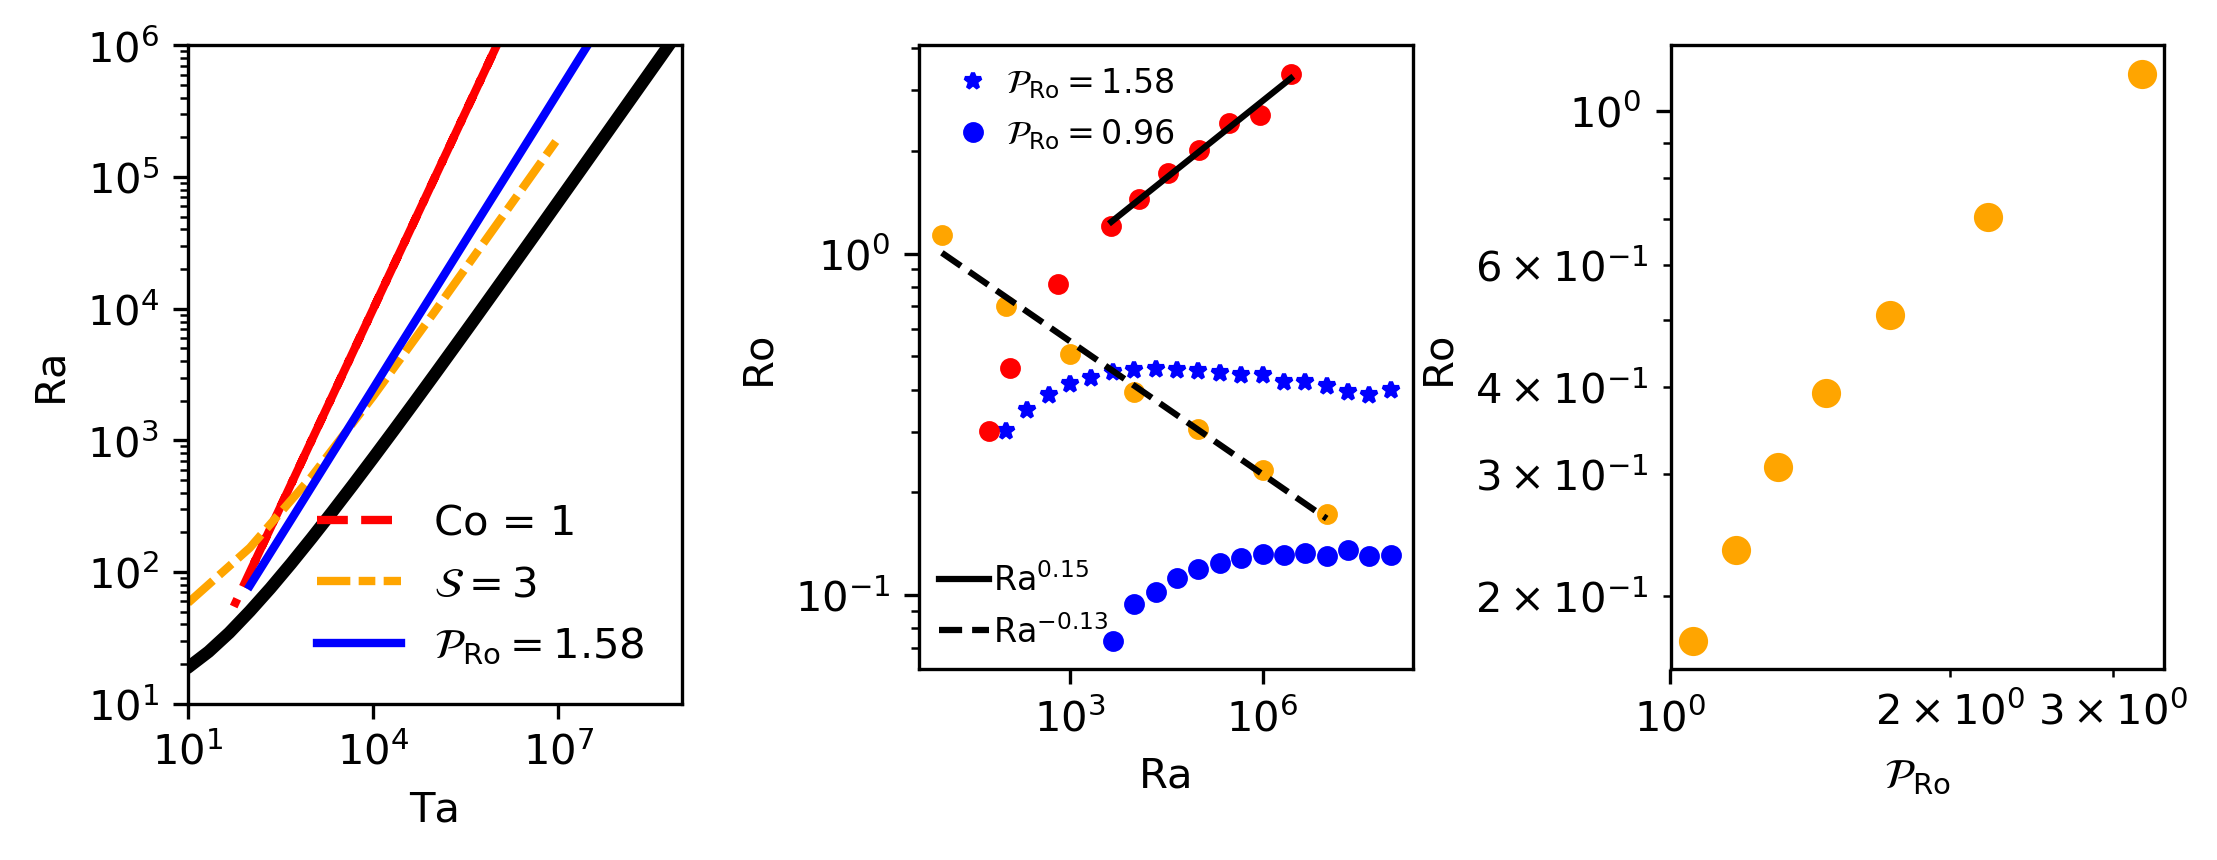
\includegraphics[width=\textwidth]{./figs/parameter_space.png}
\caption{(a) The critical Rayleigh number, as a function of the Taylor number, 
is plotted as a solid black line. Paths of constant Convective Rossby Number
(red dashed line), constant supercriticality (orange dashed line), and 
COPRIME (blue solid line) are shown through parameter space. (b) Evolved
Rossby number is plotted vs. Taylor number along multiple constant COPRIME
paths, such as the solid blue line in (a). 
After a sharp increase at low Ta, the evolved Rossby number flattens
out and stays nearly constant across orders of magnitude of Ta.
\label{fig:parameter_space} }
\end{figure}



\section{Results \& Discussion}
\label{sec:results}
This is where figures go and other important things that we like to talk about.


\begin{figure}[h]
%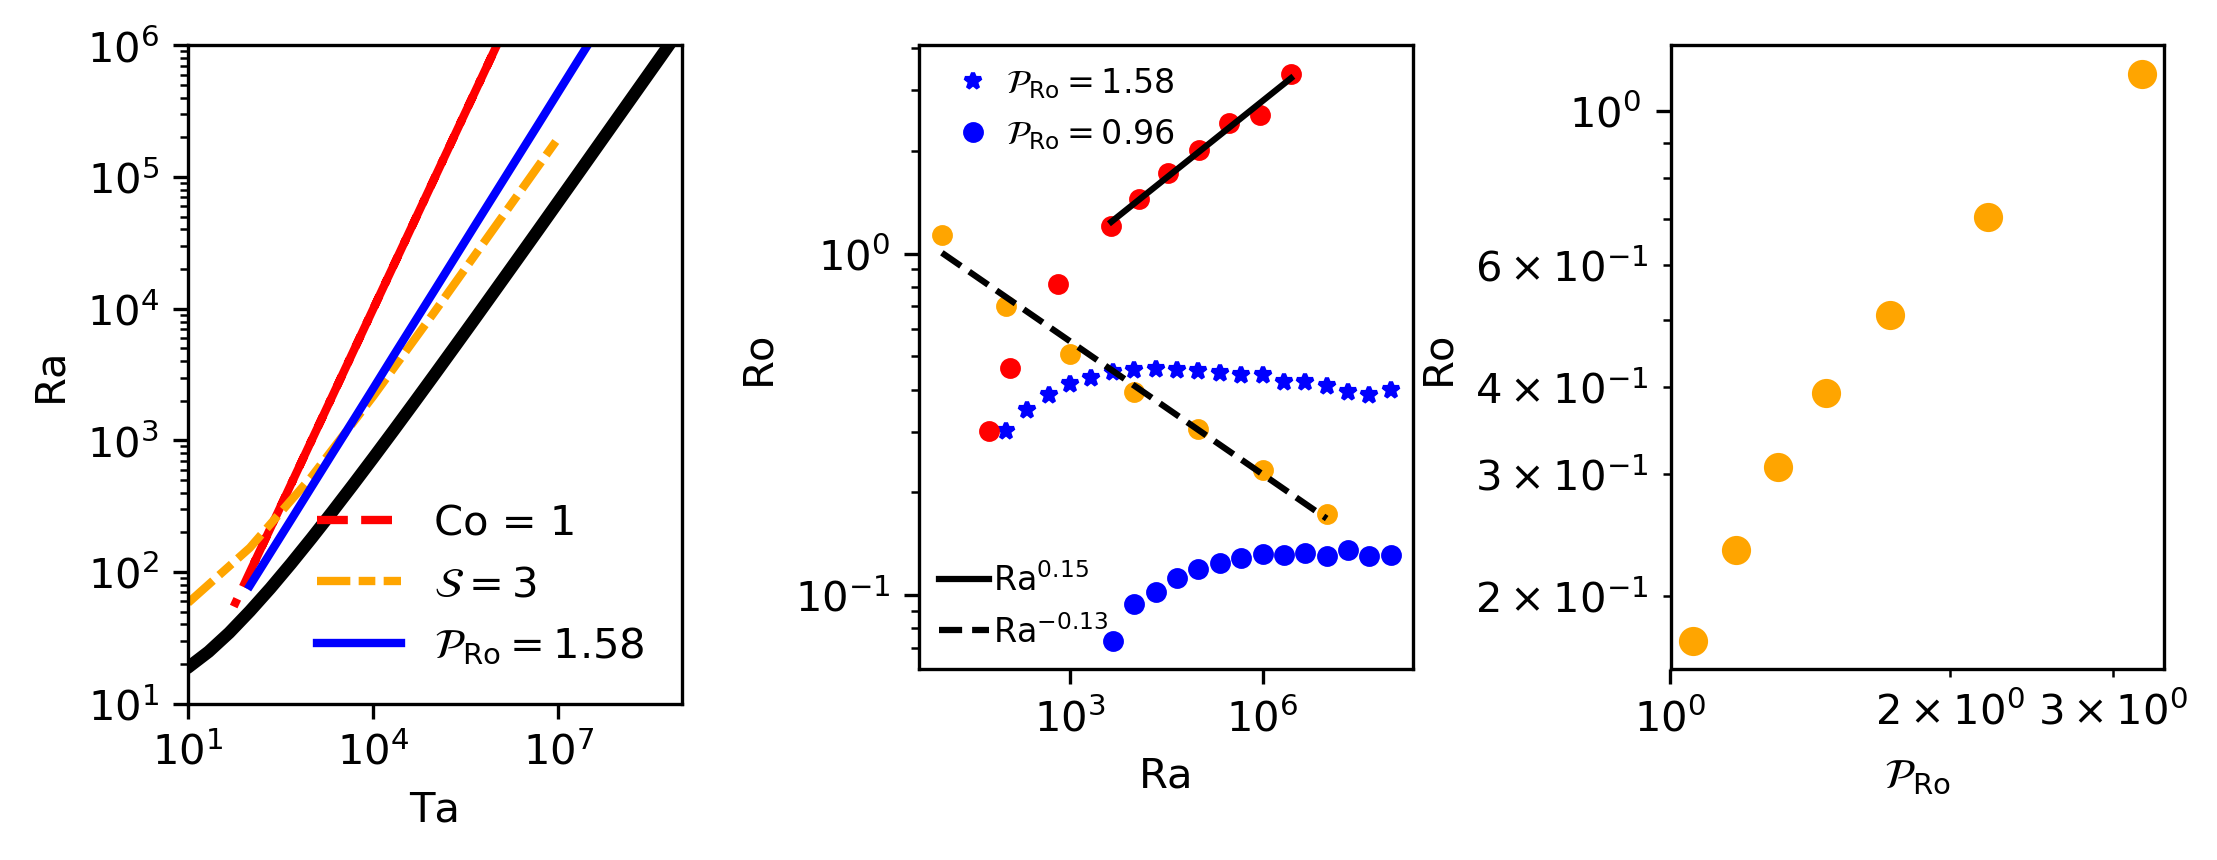
\includegraphics[width=\textwidth]{./figs/parameter_space.png}
\caption{(a) Evolved Nusselt number vs. Rayleigh number / Ra\_crit along constant
COPRIME paths. A classic scaling law of $Nu \propto Ra^{2/7}$ is observed.
(b) Evolved Reynolds number vs. Rayleigh number / Ra\_crit along constant COPRIME paths.
A classic scaling law of $Re \propto Ra^{1/2}$ is observed. These laws are
reminiscent of standard scaling laws of Re and Nu in non-rotational convection
(SOURCES SOURCES SOURCES). This suggests that at fixed Rossby number on
a constant COPRIME path (Fig. \ref{fig:parameter_space}), varying the Rayleigh
number affects the evolved dynamics in a manner similar to a nonrotating fluid.
\label{fig:nu_and_re} }
\end{figure}

\begin{figure}[h]
%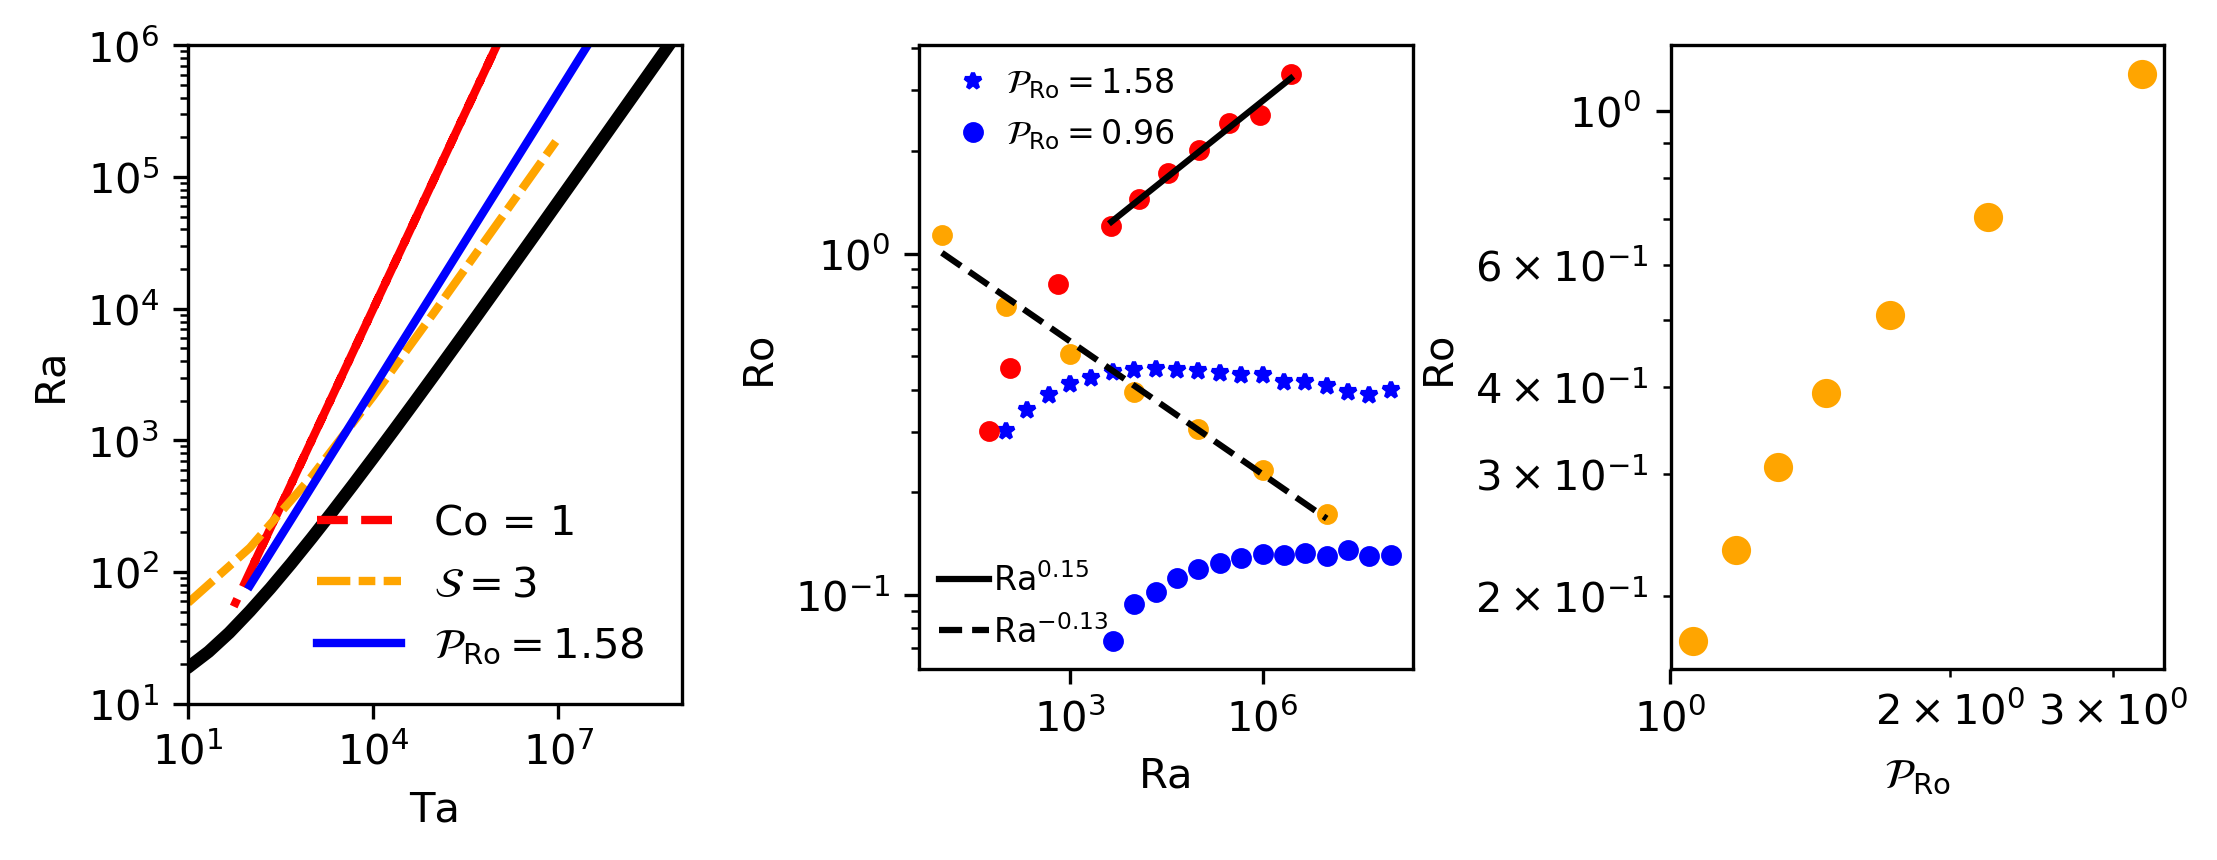
\includegraphics[width=\textwidth]{./figs/parameter_space.png}
\caption{ Here's some pretty plots, we'll figure out what we plot later.
\label{fig:pretty_convection} }
\end{figure}

\begin{figure}[h]
%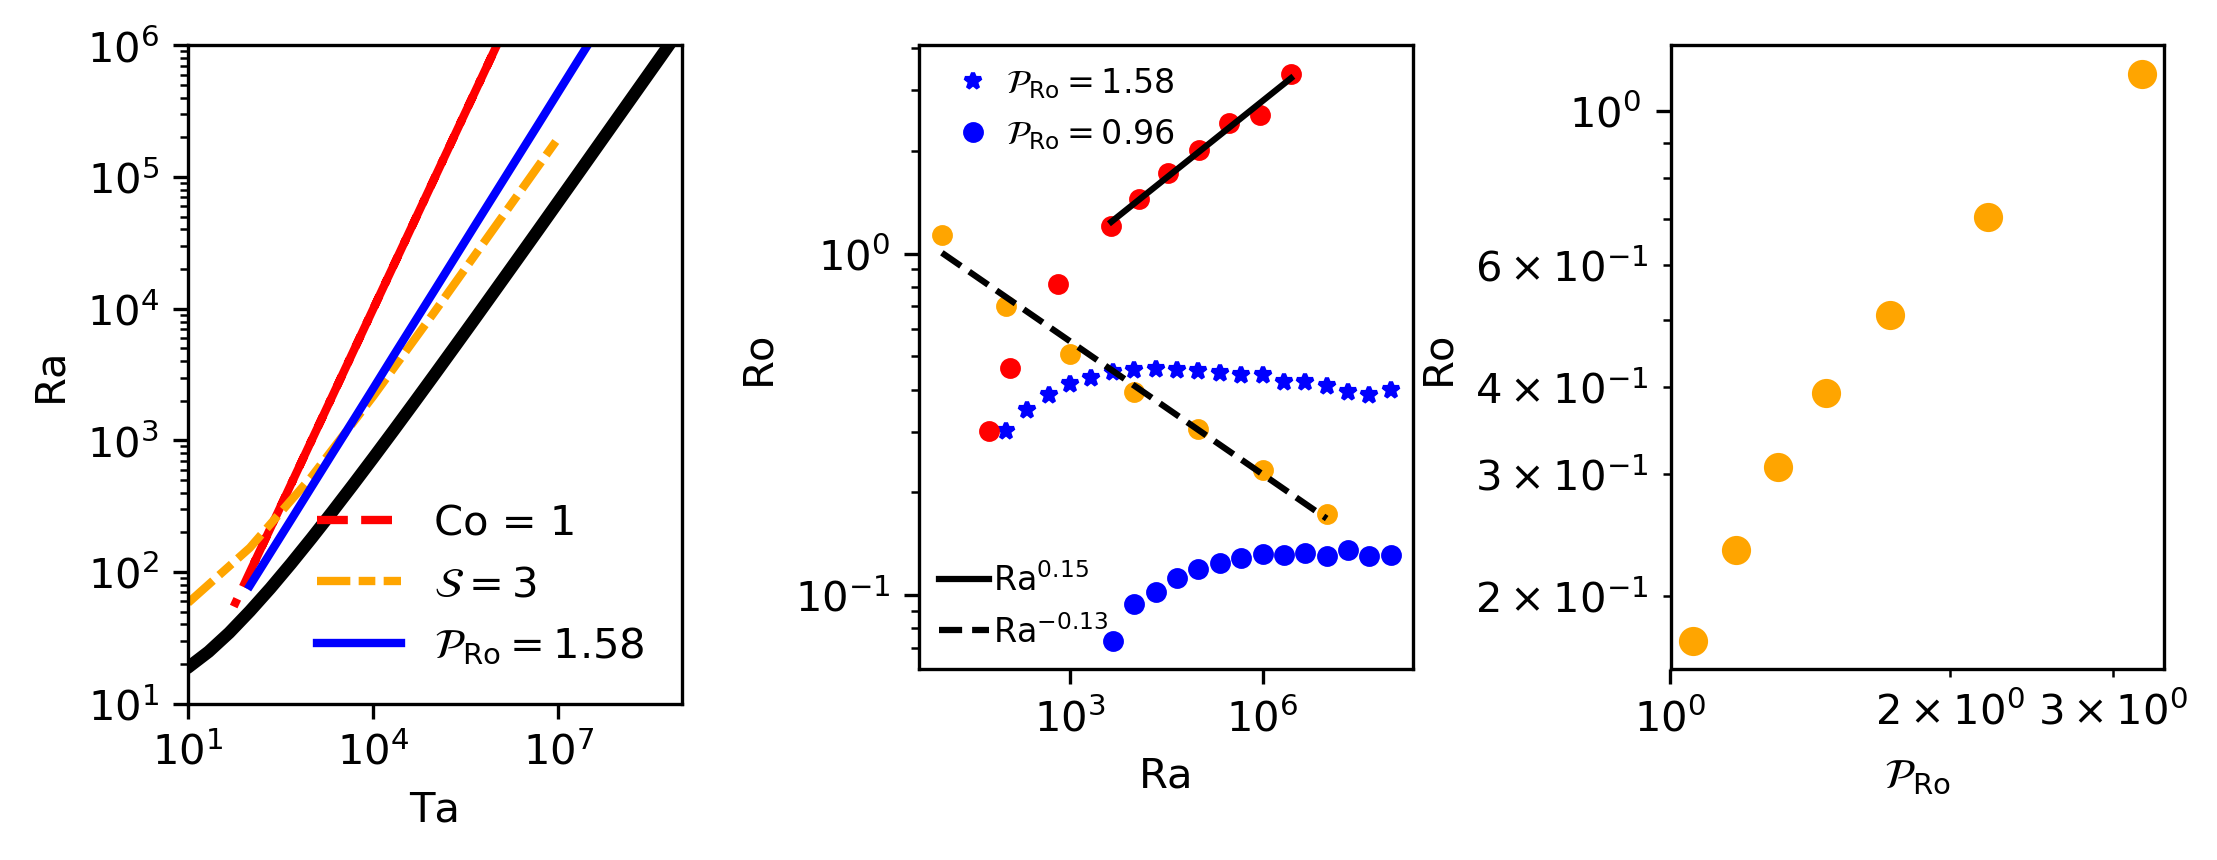
\includegraphics[width=\textwidth]{./figs/parameter_space.png}
\caption{(a) Horizontally-averaged profiles of the Rossby number are shown
vs. z for a constant COPRIME = X. (b) Horizontally-averaged profiles of 
the entropy gradient are shown vs. z for a constant COPRIME = X.
(c) Vorticity boundary layer thickness normalized by entropy boundary layer
thickness as a function of Ta/Ta\_crit for multiple COPRIME paths.
When this measure is $\gg 1$, we expect the flows to be buoyancy dominated,
when it is $\ll 1$, we expect the flows to be rotationally dominated,
and when it is $\sim 1$, we anticipate that both effects are very important.
\label{fig:profiles_and_bls} }
\end{figure}







\subsection{acknowledgements}
EHA acknowledges the support of the University of Colorado's George 
Ellery Hale Graduate Student Fellowship.
This work was additionally supported by  NASA LWS grant number NNX16AC92G.  
Computations were conducted 
with support by the NASA High End Computing (HEC) Program through the NASA 
Advanced Supercomputing (NAS) Division at Ames Research Center on Pleiades
with allocations GID s1647.
We thank  Jeff Oishi for many useful discussions. 

\bibliography{biblio.bib}
\end{document}
